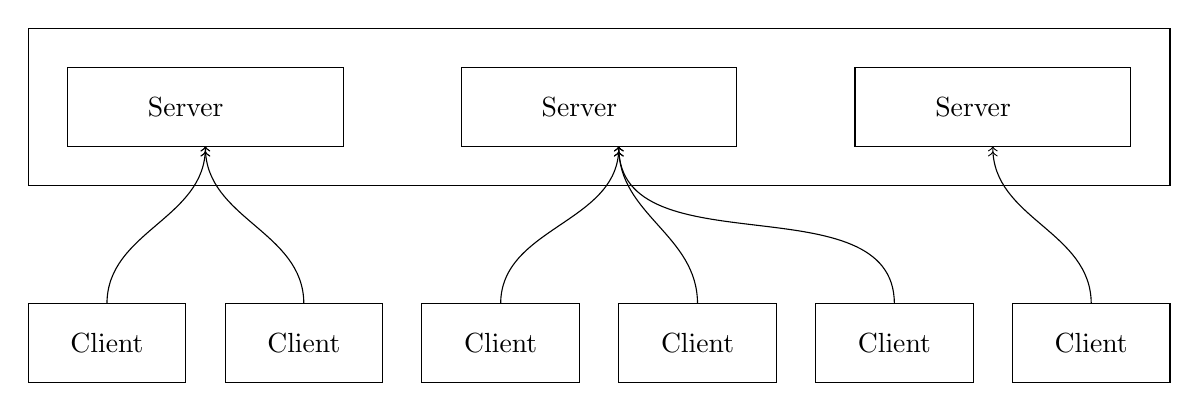
\begin{tikzpicture}
  %\draw[help lines,step=1] (-2,-2) grid (10,4);
  
  \foreach \x in {0,1,2,3,4,5}
    {
        \draw (\x*2.5,0) rectangle(\x*2.5+2,1);
        \FPeval{\result}{clip(\x+1)}
        \node at (\x*2.5+1,0.5) {Client \result};
    }
    
  \draw (0,2.5) rectangle(14.5,4.5);
  
  \foreach \x in {0,1,2}
  {
      \draw (\x*5+0.5,3) rectangle(\x*5+0.5+3.5,4);
      \FPeval{\result}{clip(\x+1)}
      \node at (\x*5+2,3.5) {Server \result};
  }
  
  \draw[->>, thin] (1,1)  to [out=90,in=-90,looseness=1] (2.25,3);
  \draw[->>, thin] (3.5,1)  to [out=90,in=-90,looseness=1] (2.25,3);

  \draw[->>, thin] (6,1)  to [out=90,in=-90,looseness=1] (7.5,3);
  \draw[->>, thin] (8.5,1)  to [out=90,in=-90,looseness=1] (7.5,3);
  \draw[->>, thin] (11,1)  to [out=90,in=-90,looseness=1] (7.5,3);
  
  \draw[->>, thin] (13.5,1)  to [out=90,in=-90,looseness=1] (12.25,3);
  
\end{tikzpicture}
